\documentclass[12pt, a4paper]{article}
\usepackage[utf8]{inputenc}
\usepackage[dvipsnames]{xcolor}
\usepackage{authblk,amsmath,amssymb,tikz,pgfplots,arydshln,array,caption,graphicx,hyperref}
\pgfplotsset{compat=newest}
\usepgfplotslibrary{patchplots,colormaps}
\usetikzlibrary{decorations.markings}

\begin{document}

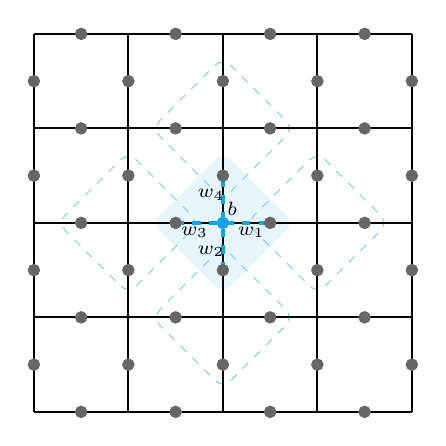
\begin{tikzpicture}[scale=0.6]
\filldraw[fill=Cerulean!10, draw=none, rounded corners] (0,-1-0.5)--(1+0.5,0)--(0,1+0.5)--(-1-0.5,0)--cycle;
\draw[Cerulean!50, dashed, rounded corners] (2,-1-0.5)--(3+0.5,0)--(2,1+0.5)--(1-0.5,0)--cycle;
\draw[Cerulean!50, dashed, rounded corners] (-2,-1-0.5)--(-1+0.5,0)--(-2,1+0.5)--(-3-0.5,0)--cycle;
\draw[Cerulean!50, dashed, rounded corners] (0,1-0.5)--(1+0.5,2)--(0,3+0.5)--(-1-0.5,2)--cycle;
\draw[Cerulean!50, dashed, rounded corners] (0,-3-0.5)--(1+0.5,-2)--(0,-1+0.5)--(-1-0.5,-2)--cycle;
\foreach \i in {-4, -2, 0, 2, 4}
        \draw[thick, black] ({\i},-4) -- ({\i},4);
\foreach \j in {-4, -2, 0, 2, 4}
        \draw[thick, black] (-4,{\j}) -- (4,{\j});
\draw[very thick, dashed, Cerulean] (-1,0) -- (1,0);
\draw[very thick, dashed, Cerulean] (0,-1) -- (0,1);
\foreach \i in {-3, -1, 1, 3}
\foreach \j in {-4, -2, 0, 2, 4}
        \filldraw[darkgray!80] ({\i},{\j}) circle (0.12);
\foreach \i in {-4, -2, 0, 2, 4}
\foreach \j in {-3, -1, 1, 3}
        \filldraw[darkgray!80] ({\i},{\j}) circle (0.12);
\filldraw[Cerulean] (0,0) circle (0.12);
\node[black] at (0.2,0.3) {\scriptsize $b$};
\node[black] at (0.6,-0.2) {\scriptsize $w_1$};
\node[black] at (-0.25,-0.6) {\scriptsize $w_2$};
\node[black] at (-0.6,-0.2) {\scriptsize $w_3$};
\node[black] at (-0.25,0.6) {\scriptsize $w_4$};
\end{tikzpicture}

\end{document}